\title[DS - Rollback-Recovery]{\textbf{Distributed Algorithms}\\Rollback-Recovery}

\begin{document}

%-------------------------------------------------------------------------
\begin{frame}
\titlepage

\invisible{
\nobibliography*{../references}
}

\end{frame}

\section{Introduction}

\begin{frame}{Reliability -- different techniques, different focus}
	
\begin{block}{Fault tolerance}
Offers the abstraction of a reliable system that tolerates faults
\BI
\item \alert{Group communication}\\
 Offers an abstraction of an ideal communication system that simplifies the development of reliable applications
\EI
\end{block}
\begin{block}{Fault-recovery}
Once a fault occurs, we want to recover to a previous correct state
\BI
\item \alert{Transactions}\\
  Data-oriented application	
\item \alert{Rollback-recovery}\\
Long-running applications such as scientific computing, where failures are rare but process state is important
\EI 
\end{block}
\end{frame}


\begin{frame}{The idea}
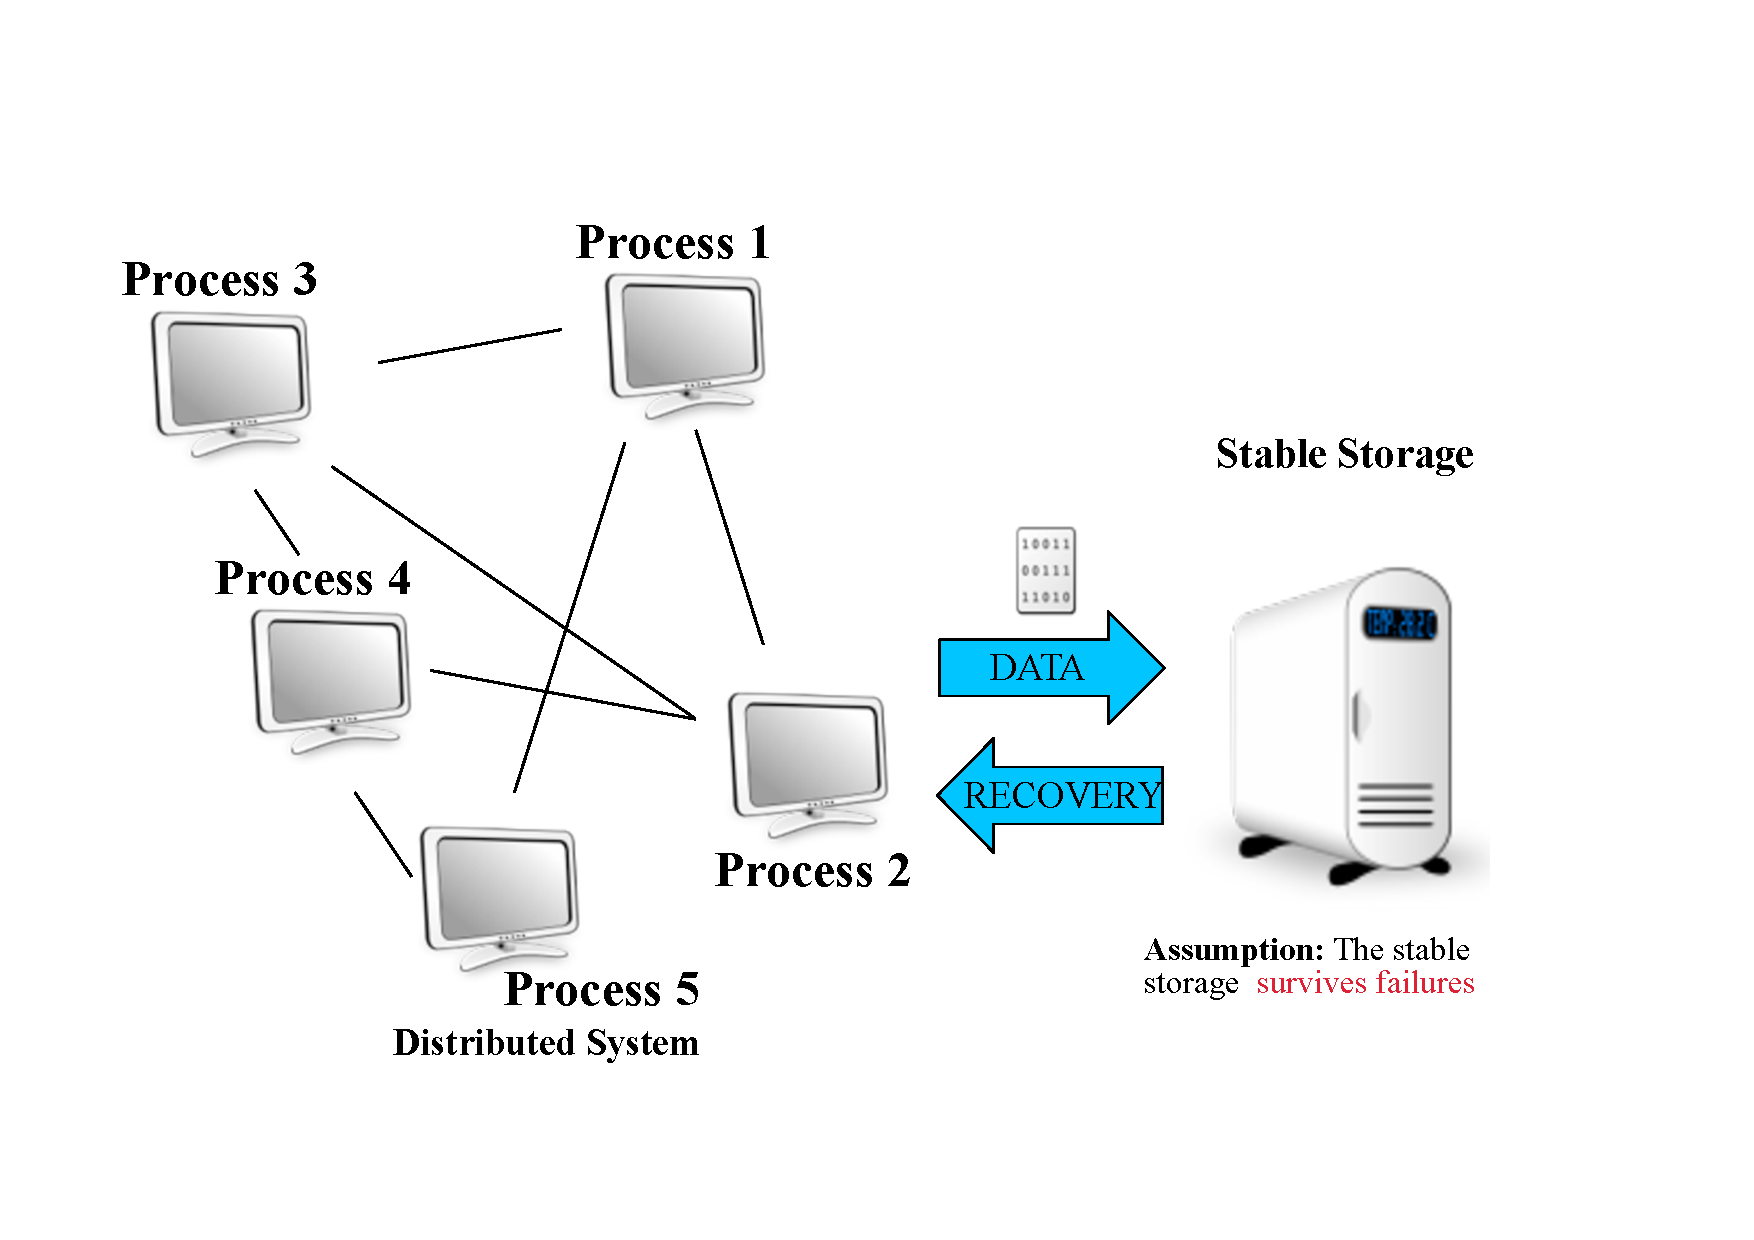
\includegraphics[width=\textwidth]{figs/16/rr-idea}
\end{frame}

\begin{frame}{The idea}
	
\BIL
\item \alert{Processes}:
\BI
\item have access to a stable storage that survives all tolerated failures 
\item disks, RAID arrays
\EI
\item \alert{Stable storage}:
\BI
\item is used to save recovery information periodically during failure-free periods.
\EI
\item \alert{Upon a failure}:
\BI
\item a failed process uses the saved information to restart the computation from an intermediate state, thereby reducing the amount of lost computation
\EI
\EIL
\end{frame}

\section{Background and definition}

\subsection{System model}

\begin{frame}{System model}

\begin{block}{Processes}
\BI
\item Fixed number $N$ of processes 
\item Process failures
\BI
\item Fail-stop model
\item Volatile memory is lost
\item Access to stable storage that survives failures
\EI
\EI
\end{block}
\begin{block}{Communication}
\BI
\item No partitioning
\item Different models:
 \BI 
  \item Unreliable channels (lose, duplicate, reorder) 
  \item Reliable channels (FIFO)
 \EI
\item Different protocols for different models
\EI
\end{block}
\end{frame}

\begin{frame}{System model}
\begin{block}{Determinism vs non-determinism}
\BIL
\item State-intervals, each started by a non-deterministic event
\item Execution during each state interval is deterministic
\item \alert{PieceWise deterministic} assumption (PWD)\\
\emph{
It is possible to capture sufficient information about non-deterministic events that initiate the state intervals
}
\EIL
\end{block}
\begin{figure}
	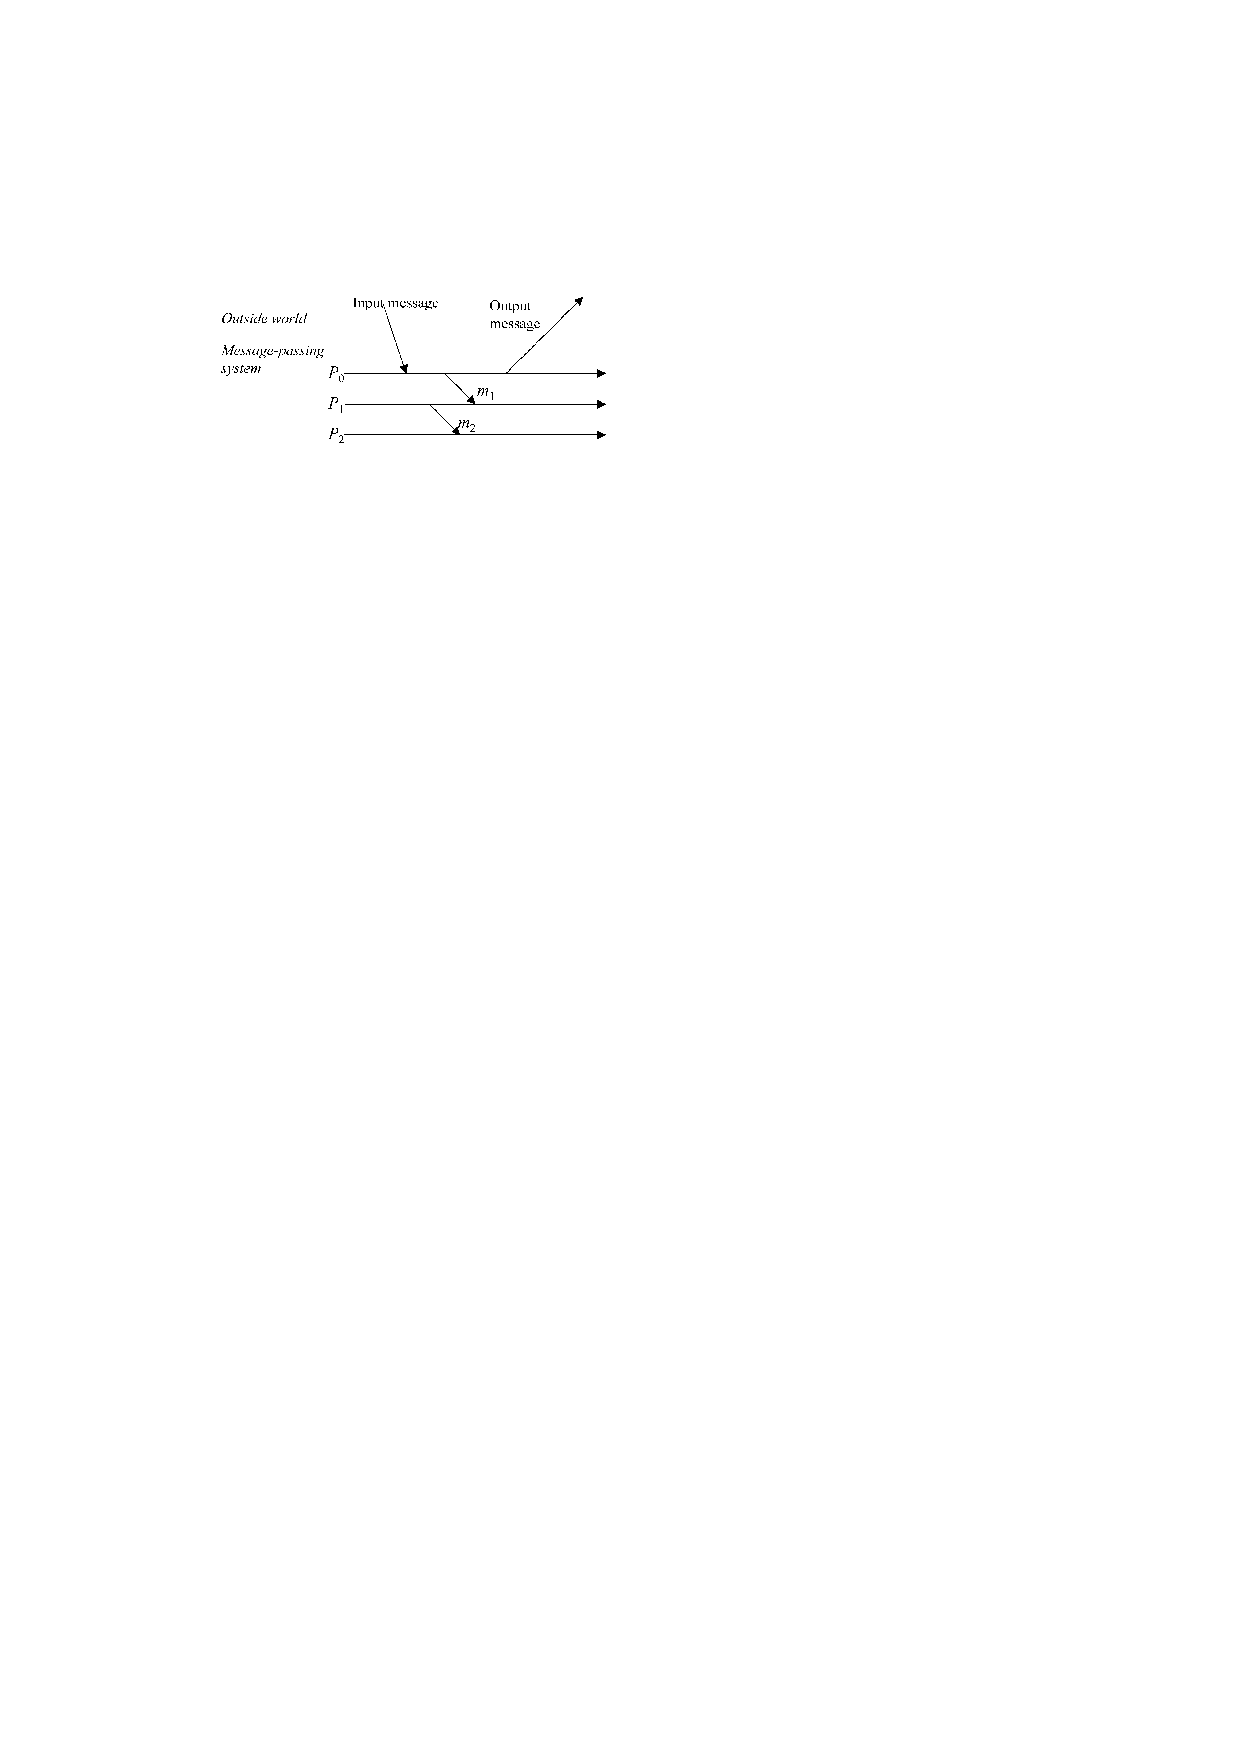
\includegraphics[width=0.6\textwidth]{figs/16/system}
\end{figure}	

\end{frame}

\subsection{Saving state}


\begin{frame}{Correctness condition}
\begin{block}{Correctness}
A system recovers correctly if its internal state after the recovery is consistent with the observable behavior of the system before the failure.
\end{block}
\bigskip
\BI
\item Rollback-recovery protocols therefore must persist information
\BI
\item about the internal interactions among processes 
\item the external interactions with the outside world
\EI
\EI
\end{frame}

\begin{frame}{Basic approaches}
	
\begin{block}{Checkpointing}
\BI
\item Store the states of the participating processes, called checkpoints 
\EI
\end{block}
\begin{block}{Message/event logging}
\BI
\item Log messages exchanged among the processes 
\item Log interactions with input and output devices
\item In general, log events that occur at each process	
\EI
\end{block}	
\end{frame}

\begin{frame}{An hybrid approach}
\BIL
\item \alert{When executing}
\BI
\item Make a periodic “big” checkpoint
\item More frequently, make incremental additions
\EI
\item \alert{When recovering}
\BI
\item Restore latest checkpoint
\item Replay messages/events stored in logs
\item Combining checkpoints with message logging makes it possible to restore a state that lies beyond the most recent checkpoint
\EI
\EIL
\end{frame}

\begin{frame}{How to save the state -- ask the application}
	
\BIL
\item \emph{A checkpoint should include data that can't be regenerated
in a quick, straightforward way}
\item Some applications might have massive data structures while they run
\BI
\item ... some of them may have been read from the disk at startup
\item ... some of them may rarely be changed
\item ... some of them may have been generated on the fly
\EI
\item Example: scientific computing
\EIL
\end{frame}

\begin{frame}{How to save the state -- transparently}
\BIL
	\item  \emph{A checkpoint should include the entire state of a process/system}
		\BI
		\item Write out its memory “layout”
		\item Contents of all pages
		\item Contents of registers
		\EI
	\item Resume the process by simply reloading its entire state
		\BI
		\item Windows XP, GNU/Linux OSs do this for “hibernate” feature
		\item Virtual machines
		\EI
	\item Potentially, very fast
\EIL
\end{frame}

\begin{frame}{How to save the state}
\BIL
	\item How (not) to take a checkpoint
		\BI
		\item Block execution, save entire process state to stable storage
		\item Very high overhead during failure-free execution
		\item Lots of unnecessary data saved on stable storage
		\EI
	\item How to take a checkpoint
	\BI
		\item Take checkpoints incrementally
			\BI
			\item Save only pages modified since last checkpoint
			\item Use “dirty” bit to determine which pages to save
			\EI
		\item Save only “interesting” parts of address space
			\BI
			\item Use application hints or compiler help to avoid saving useless data (e.g. dead variables)
			\EI
		\item Do not block application execution during recovery
			\BI
			\item Copy-on-write	
			\EI
	\EI
\EIL	
\end{frame}

\begin{frame}{How to save state}
\BIL
\item Problem: a program with a bug can...
\begin{enumerate}
\item Crash due to a corrupt data structure
\item Roll back until the last checkpoint
\item Reload the same (still corrupt) structure
\item ... goto 1
\end{enumerate}
\item “Rebuilding” data structures from scratch avoid this risk
\EIL
\end{frame}

\subsection{Stable storage}

\begin{frame}{Stable storage}
	
\BIL
\item Do not confuse it with the disk storage (frequently) used to implement it.
\item Abstraction
\BI
\item Recovery data must persist through the tolerated failures and the their corresponding recoveries
\EI
\item Implementations
	\BI
	\item Tolerating a single failure
		\BI
		\item Volatile memory of another process
		\EI
	\item Tolerating transient failures
		\BI
		\item Local disk at each host
		\EI
	\item Tolerating non-transient failures
		\BI
		\item Persistent medium outside the host on which a process is running
		\EI
	\EI
\EIL
\end{frame}

\begin{frame}{Consistent global checkpoint}

\begin{columns}
\begin{column}{0.48\textwidth}
\begin{block}{\alert{Local checkpoint}}
A snapshot of a local state of a process
\end{block}
\end{column}
\begin{column}{0.48\textwidth}
\begin{block}{\alert{Global checkpoint}}
A set of local checkpoints, one from each process
\end{block}
\end{column}
\end{columns}

\begin{block}{\alert{Consistent global checkpoint}}
A global checkpoint such that no message is sent by a process after taking its
local checkpoint, that is received by another process before taking its local
checkpoint
\end{block}
\begin{figure}
	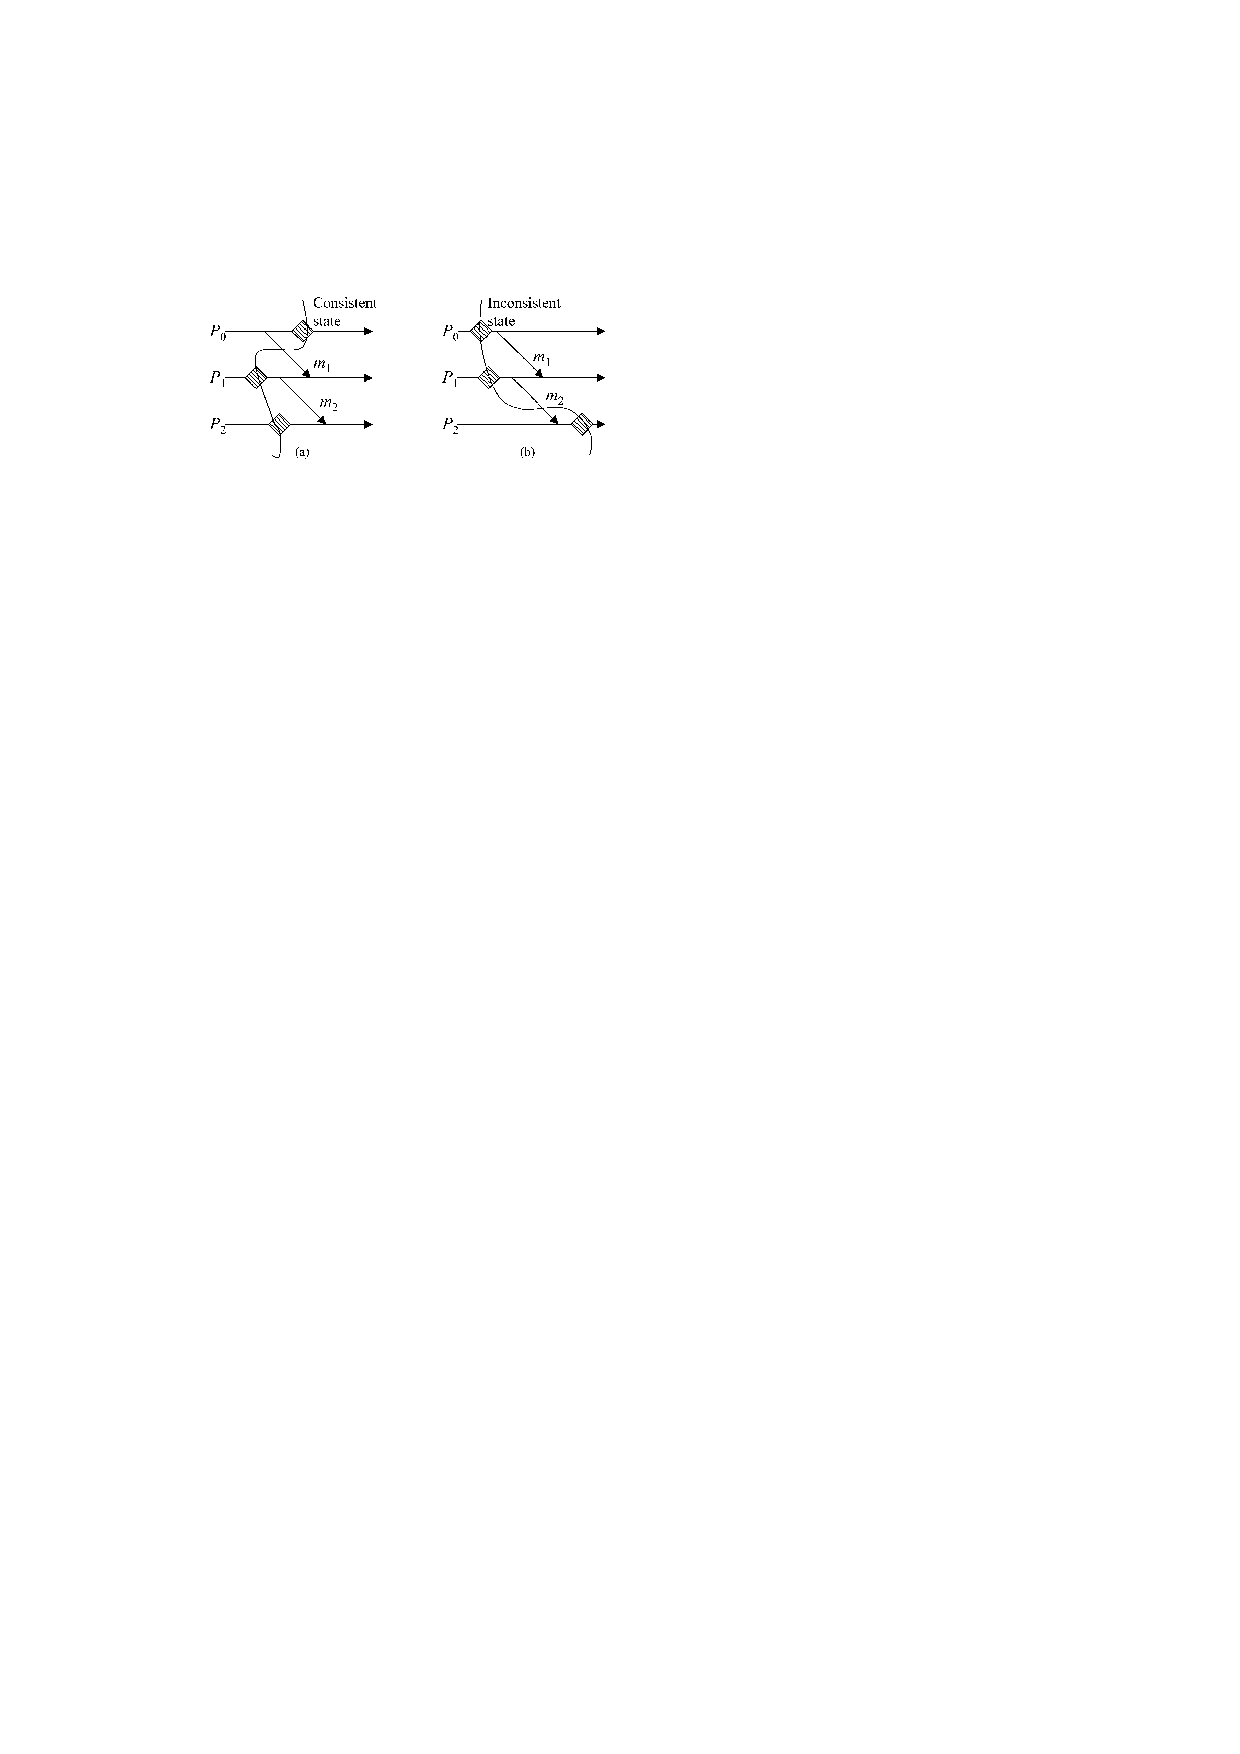
\includegraphics[width=0.5\textwidth]{figs/16/consistent}
\end{figure}
\end{frame}

\begin{frame}{Type of messages}

\begin{overprint}
\onslide<1-2>
\begin{block}{\alert{In-transit messages}}
\BI
\item Messages sent, not yet received before recovery line
\item No problem with global state consistency
\item Can be lost or delayed
\EI
\end{block}
\onslide<3-4>
\begin{block}{\alert{Lost messages}}
\BI
\item Send not undone, receive undone
\item Lost messages must be replayed
\item If implemented over
	\BI 
	\item unreliable communication, application is responsible
	\item reliable communication, recovery algorithm is responsible
	\EI
\EI
\end{block}
\onslide<5-6>
\begin{block}{\alert{Delayed messages}}
\BI
\item Messages whose receive is not recorded because the receiving process was
either down or the message arrived after the rollback of the receiving process
\EI
\end{block}
\onslide<7>
\begin{block}{\alert{Orphan messages}}
\BI
\item Send undone, receive not undone
\item To be avoided if we want consistent global states
\item No examples here
\EI
\end{block}
\onslide<8>
\begin{block}{\alert{Duplicate messages}}
\BI
\item Duplicate messages arise due to message logging and replaying during process recovery
\item Example: $m_5$ will be replayed, so it can arrive twice at $P_3$
\EI
\end{block}

\end{overprint}

\begin{overprint}
\onslide<1>
\begin{figure}
	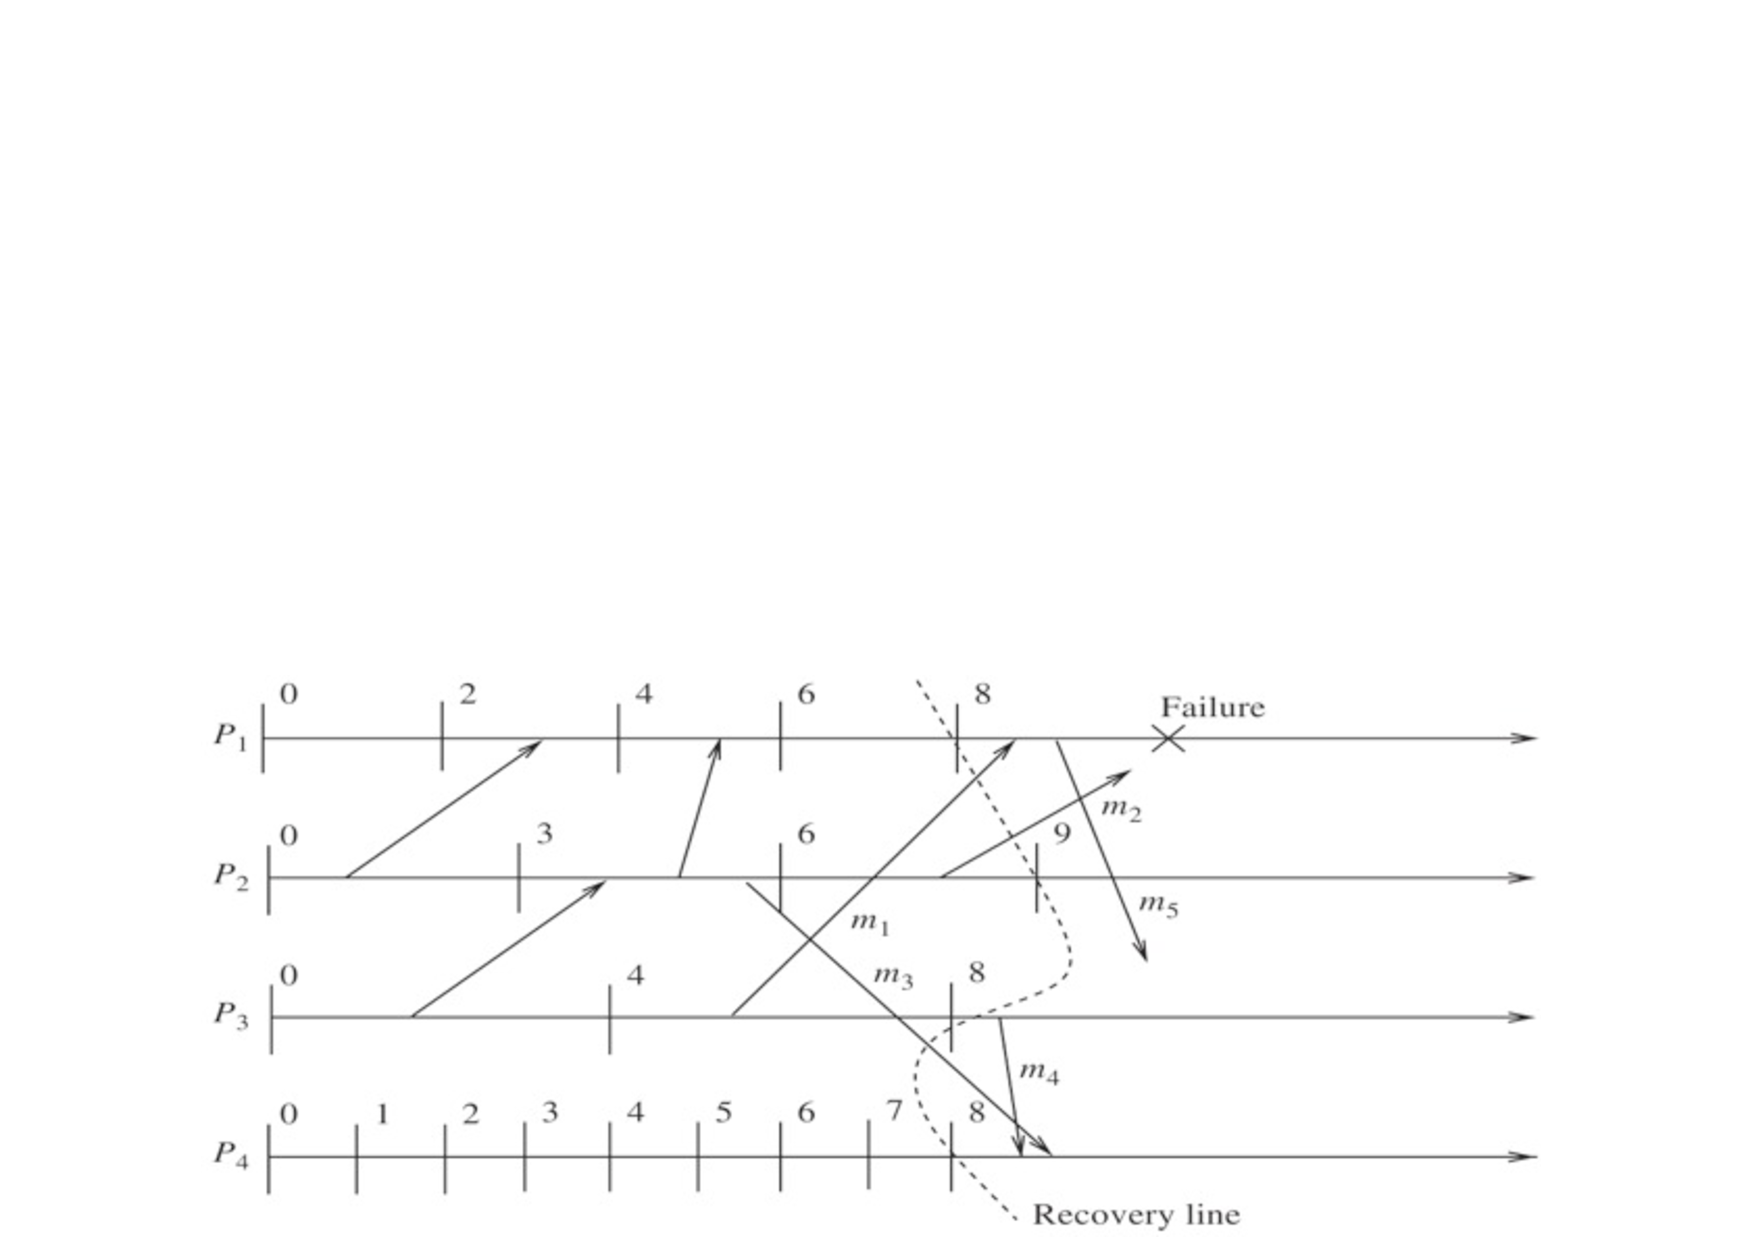
\includegraphics[width=0.7\textwidth,page=1]{figs/16/messages}
\end{figure}
\onslide<2>
\begin{figure}
	\includegraphics[width=0.7\textwidth,page=2]{figs/16/messages}
\end{figure}
\onslide<3>
\begin{figure}
	\includegraphics[width=0.7\textwidth,page=3]{figs/16/messages}
\end{figure}
\onslide<4>
\begin{figure}
	\includegraphics[width=0.7\textwidth,page=4]{figs/16/messages}
\end{figure}
\onslide<5>
\begin{figure}
	\includegraphics[width=0.7\textwidth,page=5]{figs/16/messages}
\end{figure}
\onslide<6>
\begin{figure}
	\includegraphics[width=0.7\textwidth,page=6]{figs/16/messages}
\end{figure}
\onslide<7>
\begin{figure}
	\includegraphics[width=0.7\textwidth,page=7]{figs/16/messages}
\end{figure}
\onslide<8>
\begin{figure}
	\includegraphics[width=0.7\textwidth,page=7]{figs/16/messages}
\end{figure}

\end{overprint}


\end{frame}

\begin{frame}{}
\end{frame}
\begin{frame}{}
\end{frame}


%%%%%%%%%%%%%%%%%%%%%%%%%%%%%%%%%%%%%%%%%%%%%%%%%%%%%%%%%%%%%%%%%%%%%%%%%%
\section{Bibliography}

%-------------------------------------------------------------------------
\begin{frame}{Reading material}

{\footnotesize
\BIL
\item \bibentry{alvisi-rr}
\EIL
}

\invisible{{\tiny
\bibliographystyle{abbrv}
\bibliography{../references} 
}}

\end{frame}

\end{document}